\newpage
\section{Ergebnisse}
\label{sec:ergebnisse}
%5.) Inhalt des Kapitels: „Ergebnisse und Resultate
%- Darstellung der eigenen Versuchsergebnisse in Sätzen in Kombination mit
%entsprechenden Tabellen (u.a. aus Messprotokoll) und Abbildungen bzw. grafischer
%Darstellung der Ergebnisse.
%- Alle Abbildungen und Tabellen sind durchzunummerieren (Abb. 01, …, Tabelle 01: …)
%und mit einer Bild- bzw. Tabellenunterschrift zu versehen.
%- Der Inhalt von Abbildungen, z.B. der Verlauf eines Graphen, ist jeweils im Text zu
%erläutern und kurz zu beschreiben. Beschreibung der Verläufe von Funktionen bzw.
%der Graphen im Text unter Verweis auf die Abbildung bzw. Abbildungsnummer und
%Herausarbeitung ihrer „Kernaussage“ und Ursache bzw. Hintergründe besonderer
%„Verläufe“.
%- Rechenwege mit denen die experimentellen Daten für die Auswertung bearbeitet
%wurden bzw. der Gang der Auswertung muss vollständig beschrieben und für einen
%Leser nachvollziehbar sein.
\subsection*{Bestimmung der Stoffmengenanteile mittels Kalibrierung}
Zur Bestimmung der Ethanolanteile werden die gemessenen Brechungsindices, der flüssigen und gasförmigen Phase, mit Hilfe einer Kalibrierfunktion umgerechnet. Diese bestimmt sich durch die quadratische Regression der Daten, welche in der Versuchsanleitung gegeben sind. Gleichung \eqref{gl:reg} ist somit die Umrechnungsgleichung des Brechungsindexes in den jeweiligen Ethanol-Anteil.
\begin{flalign}
\label{gl:reg}
x_{\text{Ethanol}} (n)&= -97,53*n^2+256,05*n-166,86
\end{flalign}
Die sich daraus ergebenden Anteile sind in Tab. \ref{tab:zusammensetzung} aufgeführt. Es ist zuerkennen, dass die Werte für reines Ethanol und reines Cyclohexan nicht \SI{100}{\percent} entsprechen. Gründe hierfür könnten durch Messfehler verursacht werden und sollten in einer wiederholten Messung untersucht werden. Diese Abweichungen könnten die nachfolgenden Untersuchen und Schlussfolgerungen signifikant beeinflussen.
% Table generated by Excel2LaTeX from sheet 'Data'
\begin{table}[h!]
	\renewcommand*{\arraystretch}{1.2}
	\centering
	\caption{Brechungsindices und Zusammensetzungen der Flüssig- und Dampfphasen in Abhängigkeit von der Temperatur}
	\resizebox{15cm}{!}{
		\begin{tabular}{c|c|cc|cc|cc}
			\hline
			\textbf{Nr.} & $\boldmath T \left[\si{\celsius}\right]$ & $\boldmath n_{L} \left[-\right]$ &$\boldmath n_{V} \left[-\right]$ &$\boldmath x_{\text{\textbf{Ethanol}}}^L \left[-\right]$ &$\boldmath x_{\text{\textbf{Ethanol}}}^V \left[-\right]$ &$\boldmath x_{\text{\textbf{Cyclohexan}}}^L \left[-\right]$ &$\boldmath x_{\text{\textbf{Cyclohexan}}}^V \left[-\right]$ \\
			\hline
			1     & 78,709 & 1,359 & 1,358 & 0,996 & 1,005 & 0,004 & -0,005 \\
			2     & 74,350 & 1,360 & 1,375 & 0,987 & 0,826 & 0,013 & 0,174 \\
			3     & 71,380 & 1,365 & 1,383 & 0,938 & 0,723 & 0,062 & 0,277 \\
			4     & 69,444 & 1,368 & 1,387 & 0,907 & 0,667 & 0,093 & 0,333 \\
			5     & 68,168 & 1,371 & 1,391 & 0,873 & 0,607 & 0,127 & 0,393 \\
			6     & 67,277 & 1,374 & 1,393 & 0,838 & 0,576 & 0,162 & 0,424 \\
			7     & 66,160 & 1,381 & 1,395 & 0,750 & 0,545 & 0,250 & 0,455 \\
			8     & 77,996 & 1,423 & 1,42  & 0,019 & 0,082 & 0,981 & 0,918 \\
			9     & 73,657 & 1,422 & 1,413 & 0,040 & 0,224 & 0,960 & 0,776 \\
			10    & 70,381 & 1,422 & 1,408 & 0,040 & 0,319 & 0,960 & 0,681 \\
			11    & 68,180 & 1,420 & 1,406 & 0,082 & 0,356 & 0,918 & 0,644 \\
			12    & 65,943 & 1,414 & 1,402 & 0,204 & 0,427 & 0,796 & 0,573 \\
			13    & 65,374 & 1,407 & 1,401 & 0,338 & 0,445 & 0,662 & 0,555 \\
	\end{tabular}}
	\label{tab:zusammensetzung}%
\end{table}%
\FloatBarrier

\subsection*{Berechnung von Dampfdruck und Aktivitätskoeffizienten}
Die Berechnung der Dampfdrücke erfolgt nach der \textsc{Antoine}-Gleichung \eqref{gl:ant} und ist in umgestellter Form nach dem Dampfdruck in Gleichung \eqref{gl:ant_dampf} dargestellt. Die stoffspezifischen \textsc{Antoine}-Parameter sind der Versuchsanleitung zu entnehmen.
\begin{flalign}
\label{gl:ant_dampf}
p_i^0(T) \left[ \si{\kilo \pascal}\right]&= 10^{^{A-\frac{B}{C+T\, \left[\si{\celsius}\right]}}}
\end{flalign}
\newpage
Durch Umstellen der Gleichung \eqref{gl:rd} lässt sich nun mit Hilfe des Umgebungsdrucks und der ermittelten Stoffmengen Anteile, der jeweilige Aktivitätskoeffizient bestimmen. Dargestellt sind diese für Cyclohexan und Ethanol in Tab. \ref{tab:aktiv}. Die umgestellte Gleichung findet sich unter Gl. \eqref{gl:rd_um}. Der gemessene und korrigierte Umgebungsdruck belief sich im Versuch auf $p= \SI{100,841}{\kilo \pascal}$
\begin{flalign}
\label{gl:rd_um}
	\gamma_i &= \frac{p*x_i^V}{x_i^L*p_i^0(T)}
\end{flalign}

% Table generated by Excel2LaTeX from sheet 'Tabelle2'
\begin{table}[h!]
	\centering
	\renewcommand*{\arraystretch}{1.2}
	\caption{Dampfdrücke, Partialdrücke und Aktivitätskoeffizienten von Ethanol und Cyclohexan in Abhängigkeit von der Temperatur }
	\resizebox{15cm}{!}{
	\begin{tabular}{c|ccc|ccc}
		\hline
		$\boldmath T \left[\si{\celsius}\right]$ &$\boldmath p_{\text{\textbf{Ethanol}}}^0 \left[\si{\kilo \pascal}\right]$ & $\boldmath p_{\text{\textbf{Ethanol}}} \left[\si{\kilo \pascal}\right]$ & $\boldmath \gamma_{\text{\textbf{Ethanol}}} \left[-\right]$ &$\boldmath p_{\text{\textbf{Cyclohexan}}}^0 \left[\si{\kilo \pascal}\right]$ & $\boldmath p_{\text{\textbf{Cyclohexan}}} \left[\si{\kilo \pascal}\right]$ & $\boldmath \gamma_{\text{\textbf{Cyclohexan}}} \left[-\right]$ \\
		\hline
		78,709 & 102,361 & 101,345 & 0,994 & 95,315 & -0,504 & -1,322 \\
		74,350 & 85,610 & 83,295 & 0,986 & 83,300 & 17,546 & 16,203 \\
		71,380 & 75,586 & 72,908 & 1,028 & 75,819 & 27,933 & 5,942 \\
		69,444 & 69,605 & 67,261 & 1,065 & 71,235 & 33,580 & 5,069 \\
		68,168 & 65,889 & 61,210 & 1,064 & 68,336 & 39,631 & 4,566 \\
		67,277 & 63,395 & 58,084 & 1,093 & 66,367 & 42,757 & 3,977 \\
		66,160 & 60,383 & 54,958 & 1,214 & 63,962 & 45,883 & 2,869 \\
		77,996 & 99,444 & 8,269 & 4,376 & 93,262 & 92,572 & 1,012 \\
		73,657 & 83,175 & 22,588 & 6,789 & 81,505 & 78,253 & 1,000 \\
		70,381 & 72,447 & 32,168 & 11,101 & 73,426 & 68,673 & 0,974 \\
		68,180 & 65,923 & 35,899 & 6,641 & 68,362 & 64,942 & 1,035 \\
		65,943 & 59,813 & 43,059 & 3,529 & 63,503 & 57,782 & 1,143 \\
		65,374 & 58,338 & 44,874 & 2,276 & 62,312 & 55,967 & 1,357 \\
	\end{tabular}}
	\label{tab:aktiv}%
\end{table}%
\FloatBarrier	

\subsection*{Grafische Darstellung der Messergebnisse}
\begin{figure}[h!]
	\centering
	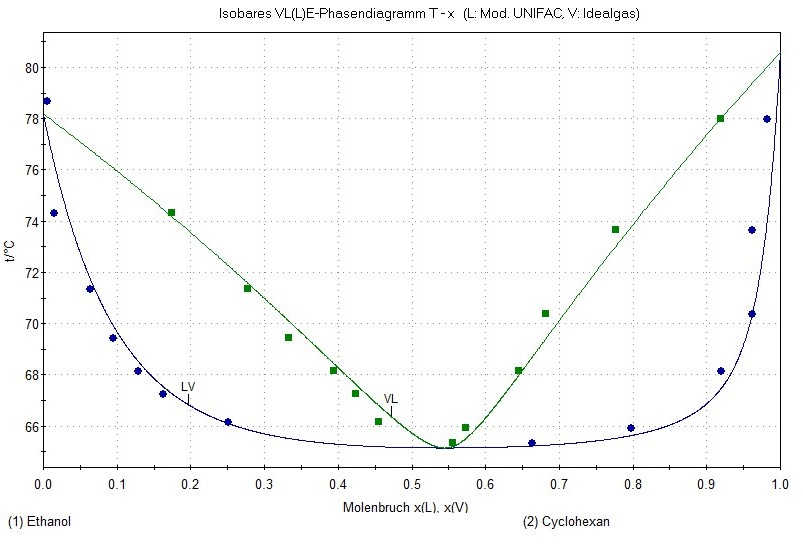
\includegraphics[width=0.75\textwidth]{img/Siededia_unifac}
	\caption{Messwerte und \textsc{UNIFAC}-Modell im Siedediagramm}
	\label{fig:siededia_unifac}
\end{figure}
\FloatBarrier
%Ende

\begin{figure}[h!]
	\centering
	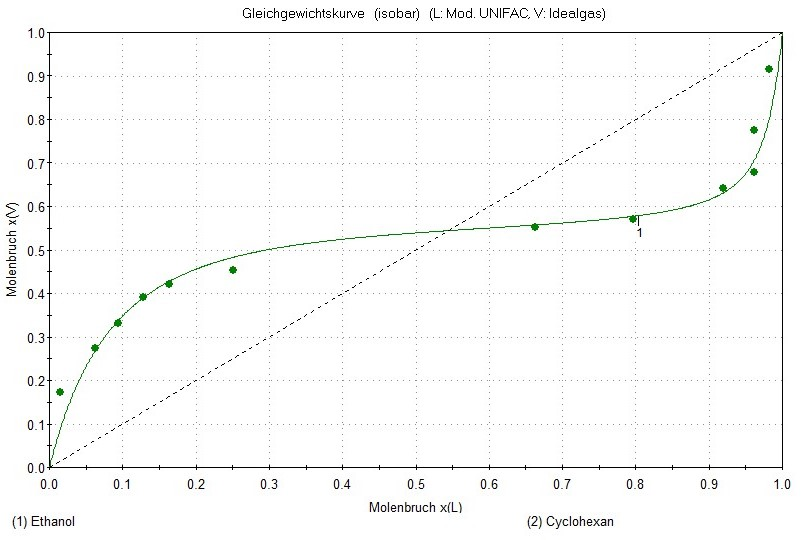
\includegraphics[width=0.75\textwidth]{img/GGW_unifac}
	\caption{Messwerte und \textsc{UNIFAC}-Modell im Gleichgewichtsdiagramm}
	\label{fig:ggw_unifac}
\end{figure}
\FloatBarrier
%Ende

\begin{figure}[h!]
	\centering
	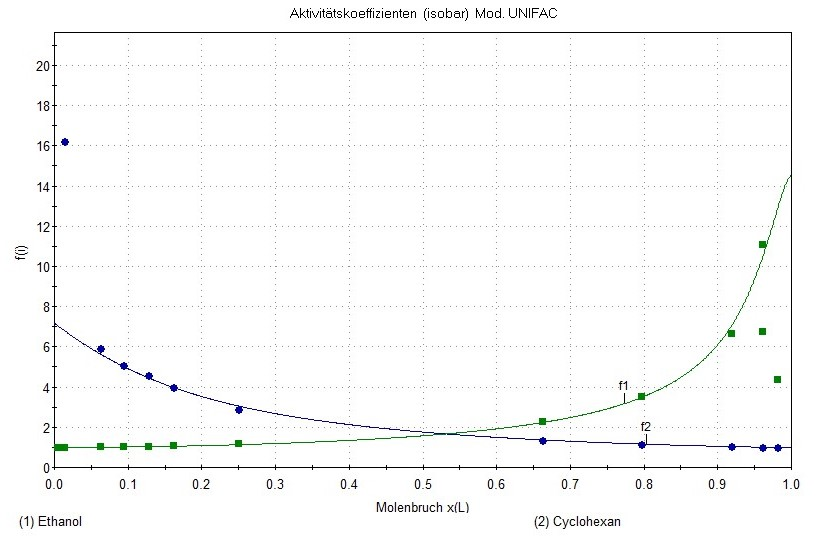
\includegraphics[width=0.75\textwidth]{img/gamma_unifac}
	\caption{Aktivitätskoeffizienten in Abhängigkeit Zusammensetzung der Flüssigphase der Messwerte und des \textsc{UNIFAC}-Modells}
	\label{fig:gamma_unifac}
\end{figure}
\FloatBarrier
%Ende

\newpage

\subsection*{Berechnung der \textsc{Wilson}-Parameter}

\begin{figure}[h!]
		\begin{center}
			\resizebox{0.8\textwidth}{!}{
				\begin{tikzpicture}[trim axis left, trim axis right]
				\begin{axis}[
				%axis lines = left,
				width = 15cm,
				height = 11cm,
				xmin = 0,
				xmax = 1,
				ymin = -3,
				ymax = 3,
				%	ytick = {-4.5,-4,...,-1},
				%	xtick = {-10,-9,...,20},
				ylabel={$\ln \left(\frac{\gamma_{_\text{Cyclohexan}}}{\gamma_{_\text{Ethanol}}}\right)$},
				%y label style={at={(0,0.5)}},
				xlabel={$x^L_{\text{Cyclohexan}}$},
				legend style={at={(0.2,0.9)},anchor=west},
				%	y dir = reverse,
				]
				\addplot [color=black, mark=*, only marks] coordinates{(0.013,2.79953475724709) (6.20000000000001E-02,1.75414600797206) (0.093,1.55974753419804) (0.127,1.45656408409239) (0.162,1.29123260877454) (0.25,0.860542364306164) (0.96,-1.91526490817348) (0.96,-2.43310546327281) (0.918,-1.85903986852428) (0.796,-1.12724160875635) (0.662,-0.517226170435867)};
				
				\addplot +[mark=none, dashed, black, domain=0:5] {-4.420173865*x+2.18036538};
				
				\legend{berechnete Punkte, Regression mit $f(x) =\SI{ -4,42}{}*x+\SI{2,18 }{}\, | \, R^2= \SI{0,9725}{}$}
				\end{axis}
				\end{tikzpicture}}
			\caption{Logarithmisches Verhältnis der Aktivitätskoeffizienten in Abhängigkeit vom Stoffmengenanteil von Cyclohexan in der Flüssigphase}
			\label{dia:wilson_linear}
		\end{center}
	\end{figure}
	\FloatBarrier
% Table generated by Excel2LaTeX from sheet 'Daten'
\begin{table}[h!]
	\renewcommand*{\arraystretch}{1.2}
	\centering
	\caption{Achsenabschnitte $n_1$ und $n_2$}
	\label{tab:abschnitt}
		%\resizebox{10.5cm}{!}{
			\begin{tabulary}{1.0\textwidth}{C|C}
				\textbf{Achsenabschnitt} & \textbf{Wert}\\
				\hline
				\textbf{$n_{\text{Ethanol}} = \gamma^\infty_{\text{Ethanol}}$} &\SI{2,18}{}\\
				\textbf{$-n_{\text{Cyclohexan}} = \gamma^\infty_{\text{Cyclohexan}}$}&\SI{2,24}{}\\
				\hline		
	\end{tabulary}
%}
\end{table}%
\FloatBarrier

\begin{flalign}
	\ln (\Lambda_{12}) + \Lambda_{21} & = 1 - \gamma^\infty_{\text{Ethanol}}\\
																			&= 1- 2,18\\
																			&= \underline{-1,18}
\end{flalign}
\begin{flalign}
\ln (\Lambda_{21}) + \Lambda_{12} & = 1 - \gamma^\infty_{\text{Cyclohexan}}\\
&= 1- 2,24\\
&= \underline{-1,24}
\end{flalign}

\begin{flalign}
	\Lambda_{12} &= 1 - \gamma^\infty_{\text{Cyclohexan}}-\ln(\Lambda_{21})\\
	\ln(\Lambda_{21})&= \ln\left(1 - \gamma^\infty_{\text{Ethanol}}-\ln(\Lambda_{12})\right)\\
	\Lambda_{12} &= 1 - \gamma^\infty_{\text{Cyclohexan}}-\ln\left[1 - \gamma^\infty_{\text{Ethanol}}-\ln(\Lambda_{12})\right]\\
								&= 1-2,24-\ln(1-2,18-\ln(\Lambda_{12}))\\
								&= -1,24-\ln(-1,18-\ln(\Lambda_{12}))\\ \tag{iterativ gelöst}
								&= \underline{0,245}
\end{flalign}

\begin{flalign}
	\Lambda_{21} &= 1 - \gamma^\infty_{\text{Ethanol}}-\ln(\Lambda_{12})\\
								&= 1- 2,18-\ln(0,245)\\
								&=\underline{0,227}
\end{flalign}

\begin{figure}[h!]
	\centering
	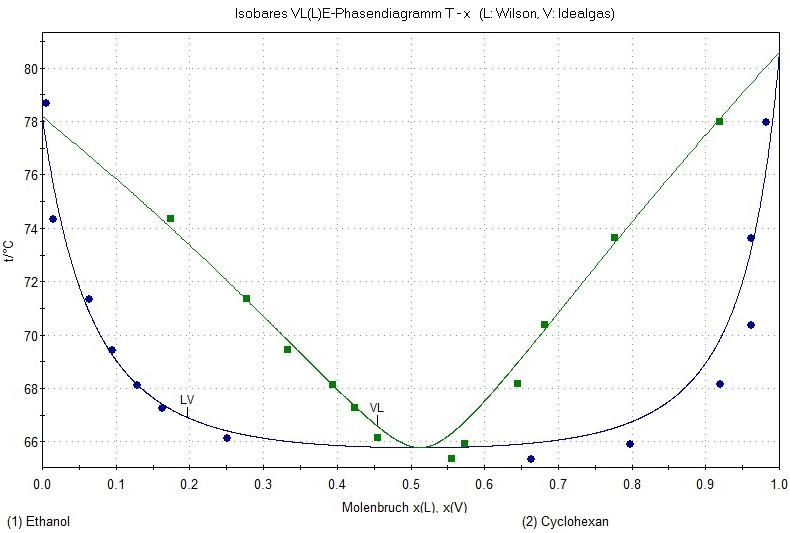
\includegraphics[width=0.75\textwidth]{img/siededia_wilson}
	\caption{Messwerte und \textsc{Wilson}-Modell im Siedediagramm}
	\label{fig:siededia_wilson}
\end{figure}
\FloatBarrier
%Ende

\begin{figure}[h!]
	\centering
	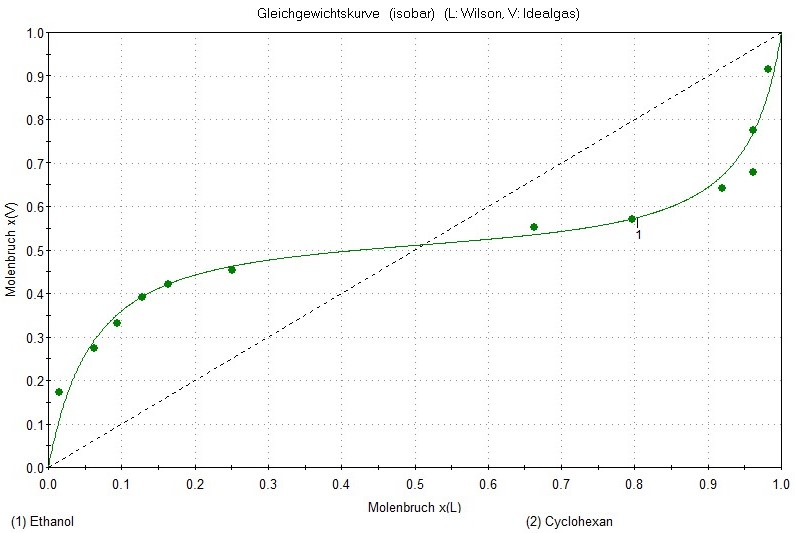
\includegraphics[width=0.75\textwidth]{img/GGW_wilson}
	\caption{Messwerte und \textsc{Wilson}-Modell im Gleichgewichtsdiagramm}
	\label{fig:ggw_wilson}
\end{figure}
\FloatBarrier
%Ende

\begin{figure}[h!]
	\centering
	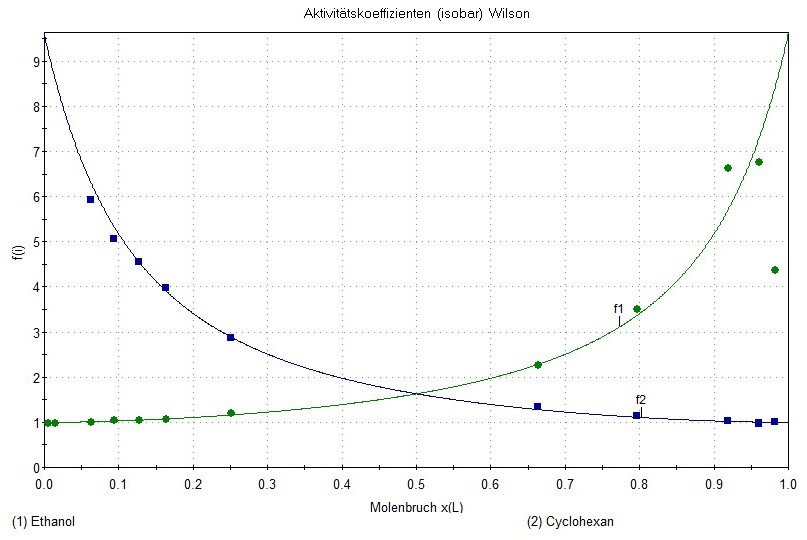
\includegraphics[width=0.75\textwidth]{img/gamma_wilson}
	\caption{Aktivitätskoeffizienten in Abhängigkeit Zusammensetzung der Flüssigphase der Messwerte und des \textsc{Wilson}-Modells}
	\label{fig:gamma_wilson}
\end{figure}
\FloatBarrier
%Ende